\chapter{Monetary Policy Objectives and Monitoring the Economy}

\fancyhead[L]{ECON0024}
\fancyhead[C]{Ch.7 Monetary Policy Objectives and Monitoring the Economy}
\fancyhead[R]{Xiaotian Tian}
\fancyfoot[L]{\hyperlink{tableofcontents}{Back to Table of Contents}}
\fancyfoot[R]{Xiaotian Tian}

\section{Basic Concepts}

    \subsection{What is a Central Bank?}
    
        \emphb{Definition}: Central banks are public (or quasi-private) institutions that manage the money supply and sometimes the banking system of a country or monetary union.

        Kay Features:
        \begin{itemize}
            \item They act as "Lenders of Last Resort" to commercial banks to prevent bankruns
            \item A key feature of modern central banks -- \emph{Independence}
            \item Some central banks are responsible for much more than monetary policy:
            \begin{itemize}
                \item Financial regulation
                \item Printing/circulating/retiring physical currency
                \item Macroprudential policy (smoothing the credit cycle)
            \end{itemize}
        \end{itemize}
        
    \subsection{What is Monetary Policy?}

        \emphb{Definition}: Monetary policy is the management of the money supply to further some economic objective(s).

        Idea behind monetary policies: by moderating money available, you can alter behaviour of agents. Monetary policy exploits \emph{trade off} between saving/borrowing and consumption.

        Monetary policy stance is usually summarised as "setting an interest rate" (sometime "policy rate"): cutting rates refers to "expansionary" while hiking rates refers to "contractionary".

        Central banks may not actually set these interest rates directly, but only \emph{target} for them: in US, the Federal Reserve targets the Federal Fund Rate (FFR) -- the average rate charged by one bank to another bank to (uncollateralised) borrow reserves at the Federal Reserve overnight. It's a market rate.

    \subsection{Transmission of Interest Rates and the Yield Curve}

        \subsubsection{Transmission}
            Monetary policy only sets/targets the overnight rate. To impact the economy, it has to be transmitted through the economy: a rise in the policy rate increases the borrowing cost of banks, so banks will charge other institutions/individuals to borrow in order to maintain their profit margins.

        \subsubsection{How Does Interest Rates Affects Economy? Consumption Euler Equation}
            Here, we discuss a simple model for intuition. Assuming log utility and perfect information (no uncertainty), we can derive the \emphb{Consumption Euler equation}:
            $$\frac{C_{t+1}}{C_t} = \beta (1+r_t) = \beta \frac{1+i_t}{1+\pi_t}$$
            where:
            \begin{itemize}
                \item $C_{t+1}, C_t$ are consumption in the corresponding period
                \item $\beta$ represents discount factor
                \item $i$ represents nominal interest rate
                \item $\pi$ represents inflation rate
            \end{itemize}
            We can see that, if the nominal interest rate $i_t$ goes up, individuals will be more willing to sacrifice their current consumption $C_t$ in exchange for higher future consumption $C_{t+1}$.

        \subsubsection{Yield Curve}
            Monetary policies changes are reflected by movements of the \emphb{yield curve}. 
            
            Overnight lending of reserves is \emph{risk-free}, but other interest rates build in a \emph{risk premium} (due to default risk, inflation risk, interest rate risk, etc.) Long-term interest rates integrate \emph{expected rates} over the duration of the loan plus \emph{risk premium} and \emph{term premium}.

            \begin{figure}[H]
                \centering
                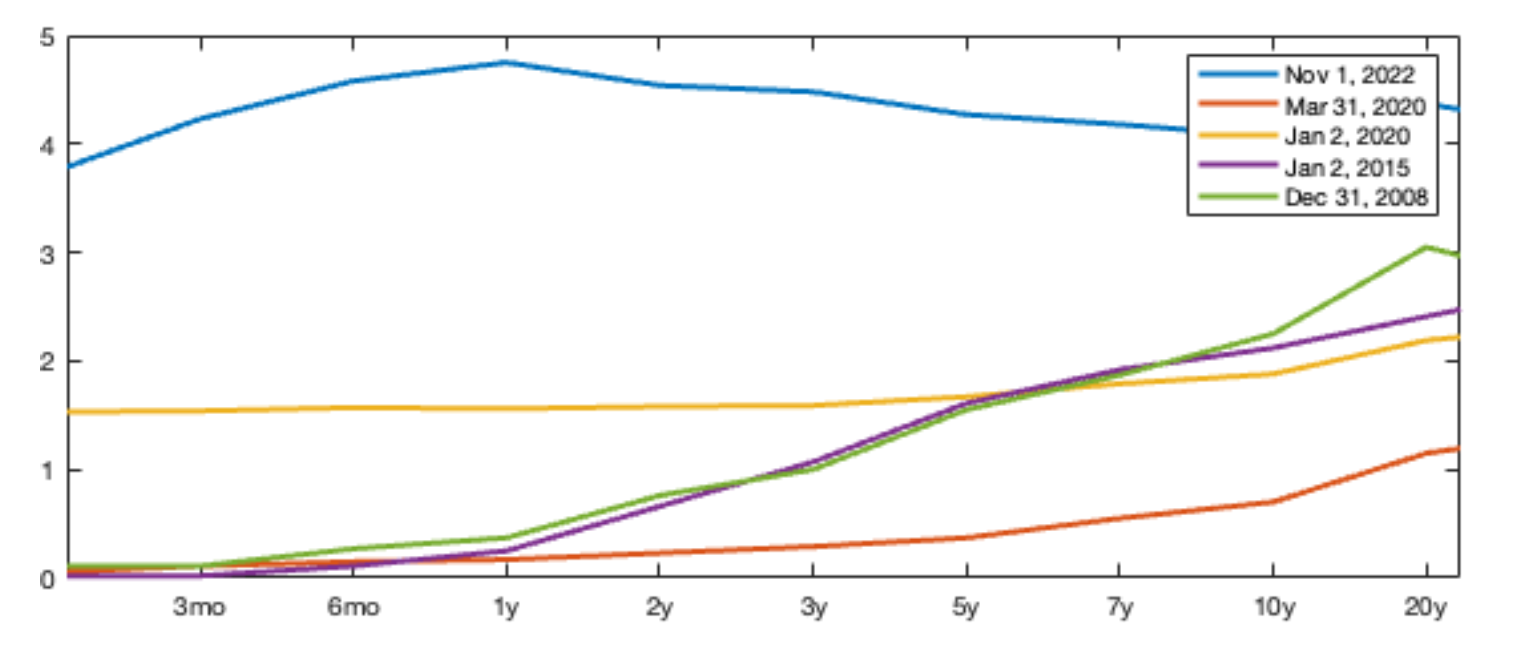
\includegraphics[width=4in]{images/ch7/yield curve.png}
                \caption{Yield Curves}
            \end{figure}

            Typically, yield curve if a healthy economy should be upward sloping due to positive risk premium and term premium. An inverted yield curve implies potential economic crisis: it predicts that the central bank will have to cut policy rate dramatically to fight recession in the future. A yield curve hitting the zero lower bound is also undesirable because it means conventional monetary policy instrument is exhausted.

         \subsubsection{Corporate Bonds?}
            The yield curves above are built upon government bonds. Corporate bonds will have higher yield curves due to default risks.
        
    \subsection{Central Bank Mandates}
    
        \subsubsection{legal Mandates and Dual Mandate Trade-off}
            Central banks are generally given very specific legal mandate:
            \begin{itemize}
                \item Bank of England: psudo dual mandate
                \begin{enumerate}
                    \item (primiary) Price stability: around 2\% inflation
                    \item (secondary) Suppot government's growth and employment objectives
                \end{enumerate}
                \item Federal Reserve: \emphb{dual mandate}
                \begin{itemize}
                    \item Maximum employment
                    \item and Stable prices (2\% inflation)
                \end{itemize}
                \item ECB: only one objective (it is too hard to accommodate business cycles of all Eurozone members)
                    \begin{itemize}
                        \item Price stability (2\% inflation)
                    \end{itemize}
            \end{itemize}

            A dual mandate necessitates a trade-off between inflation and unemployment. According to the \emphb{Neo-Keynesian Phillips Curve}:
            $$\pi_t = \beta E[\pi_{t+1}]+\kappa u_t, \kappa<0$$
            
            Any central bank with dual mandates will need to act with two conflicting objectives. Furthermore, there is a hot debate on whether we should set even more objectives for central banks, such as environment and equality.
        
        \subsubsection{Flat Philips Curve - Monetary Policy A "Solved Problem"? }
            From the mid 1990s, inflation has been stabilised around 2\% in many developed countries -- and even lower after the 2008 GFC. Some central bank started to worry about inflation being too low.

            Meanwhile, there seems to be a \empha{flat} Phillips Curve, indicating that there is no inflation-unemployment trade-off. However, on the flip side, policymakers cannot simply sacrifice employment to bring down inflation -- is today's inflation out of control?

    \subsection{Challenges to Central Bank Independence}

        Independence from political authority is a key tenet of modern central banks. Such insulation from politics allows that:
        \begin{itemize}
            \item Central banks can have long-term thinking, not in a 4-year cycle
            \item Monetary tools will not be used for political objectives (such as pumping up employment for elections)
        \end{itemize}

        When lines are blurred, inflation runs rampant, as in the Argentinean experience. However, threats to central banks' Independence were witnessed recently:
        \begin{itemize}
            \item U.S.: retaliation to perceived "mandate creep:" critics accused the Federal Reserve for going beyond its mandate. This may act as an excuse for political intervention.
            \item U.K.: the Bank of England directly purchased government bonds from the treasury. Typically, central banks buy government bonds from secondary markets to prevent the government from exploiting the "unqualified purchase" and over-expanding fiscal policies.
        \end{itemize}
        
    \subsection{Monetary Policy Implementation}

        \subsubsection{Conventional}
            The Bank of England sets the base rate directly.

            Federal Reserve and others target policy rates by conducting \emphb{Open Market Operations}: they purchase and sell government bonds on secondary markets in exchange for reserves held at the central bank to move the rate:
            \begin{itemize}
                \item Sell bonds $\leadsto$ Less reserves held by commercial banks $\leadsto$ Banks cut lending or charge higher rates
                \item Buy bonds $\leadsto$ More reserves held by commercial banks $\leadsto$ Banks lend more or charge lower rates
            \end{itemize}
            
            These transactions used to work with the minimum reserve requirement, but now on interest on reserves. Theoretically, changing interest rate paid on reserves have the same effect.

        \subsubsection{Unconventional}
            In 2008, interest rates hit the \emphb{Zero Lower Bound} (nominal IR cannot be cut lower than 0, otherwise people hold cash), but the economy was still trapped in recession, so unconventional monetary policy instruments were adopted:
            \begin{itemize}
                \item \emphb{Forward Guidance}: non-binding statements by central banks\\
                Forward guidance makes a promise about future interest rates, shifting investors' expectation of future interest rates and hence shifting the long-end of yield curve. This works theoretically but empirical evidence is unclear.
                \item \emphb{Quantitative Easing}: circumvent the yield curve / transmission and purchase bonds directly\\
                Quantitative easing purchase government bonds, corporate bonds, MBS, etc. directly. Such intervention increases demand and depress supply for those assets, so their price will increase, lowing the yield.
                \item Central Bank Information Effects?\\
                The market infer from central banks' actions. Sometime, this causes undesirable consequences: an unexpected low interest rate decision may lead the market to think about "the central bank believes the situation is worse than we evaluated."
            \end{itemize}
            
    \subsection{Stagflation}

        Current economic conditions can be characterised as \emphb{Stagflation}: the economy is stagnant with high inflation rate.

        Dilemma: for dual mandate central banks, persistently high inflation calls for more aggressive rate hikes, but such actions will push the economy into further recessions.

        Further bad news is that today's unemployment is \emph{artificially low}: since 2008, many people have dropped out of the labour force, and they are not counted as unemployed. This has been even worse since the pandemic.

    \subsection{Challenge of the Pandemic -- Supply not Demand}

        The pandemic presents a unique challenge for monetary policy: monetary policy is primarily equipped to \emph{stimulate demand}, but despite an initial drop in demand, most of post-pandemic recession was \emph{supply driven}.

        Monetary policy is not likely to have an immediate effect on supply -- no amount of interest rate cuts can alleviate lockdown at factories or reopen restaurants. Nevertheless, central banks lowered interest rates to zero immediately. (so "no one can accuse us for doing nothing")

        Because the fast pace of the pandemic recession, there is also a challenge for obtaining up-to-date data, discussed at the end of this chapter (section \ref{sec:pendamic data}).

\section{Policy Making and Data Collection}

    \subsection{The Policy Cycle}

        Central banks continuously assess the state of the economy and meet on a regular schedule to decide appropriate action.

        In both UK (Monetary Policy Committee) and US (Federal Open Market Committee), there are 8 meetings a year. Research and policy team prepare forecasts, briefings, and make recommendation to committees, and committees make policy decisions.

        Occasionally, typically during crises, unscheduled meetings are held for quicker adjustments in policies.
        
    \subsection{Collecting Data}

        Assessing the state of the economy is a major challenge due to:
        \begin{itemize}
            \item \emphb{Release Lag}: crucial macroeconomic data is often unavailable. Key releases such as GDP are only available a month after a quarter ends.
            \item \emphb{Data Vintages and Revisions}: available values of data may be inaccurate. There are at least four vintages of US GDP data, and change from the first to the fourth can be significant (the first one usually has a large error).
        \end{itemize}
        
        An aside: policymakers look at core inflation, which excludes highly volatile food and energy prices, instead of headline inflation data, but food and energy are important in the real life.
        
    \subsection{Nowcasting}

        \emphb{Nowcasting} is similar to forecasting, but with an focus on current period's data. 
        
        The idea is to infer slow releases such as GDP using quick releases for the current period. We take all data that is available for the current month/quarter, and use historical relationships to predict data that is not yet released.

        \subsubsection{Factor models and Principal Components Analysis}

            Nowcasts are typically dynamic factor models using many time series. They are a dimension reduction tool to express a big data set in terms of a few (unknown) underlying time series. Some quickly released data, such as unemployment claims, labour market reports, etc., becomes very important.

            Formally, factor models express the whole data set $X_t$ as:
            
            $$X_t = \Lambda F_t + \mu_t, \text{with}\ dim(X_t) > dim(F_t)$$

            $F_t$ here is latent / unobserved. The simplest way to estimate $\Lambda$ and $F_t$ is to find the uncorrelated factors that explain as much variations in $X_t$ as possible, which is known as \emphb{Principal Component Analysis}:

            \begin{itemize}
                \item Find the time series that explains the variations in $X_t$ the most
                \item Find a second time series that explain the variations in the residuals in $X_t$ the most, after partialing out the first factor
                \item ...
            \end{itemize}

            The number of factors/principals is determined using \emph{screen plots} or \emph{information criterion}.

            One caveat for using such principal component analysis is that estimated $\hat{F}_t$ for a fixed date $t$ depends on the sample used: different vintages of data may yield different estimates. Also, incorporating freshly released data also changes the estimates obtained from previous data.
             
        \subsubsection{Financial Data}

            While macroeconomic data comes with a delay, financial data is produced continuously. However, the challenge is that financial markets are not part of central banks' mandates, so policymakers have to infer from financial data about variables they care about. For example:

            \begin{itemize}
                \item Inferring lending conditions, which are relevant for interest rate decisions
                \item Derivatives reflect inflation expectations
                \item Yield curve reflects expectations of future economic conditions
            \end{itemize}

    \subsection{Data during the Pandemic and The Weekly Economic Index}\label{sec:pendamic data}

        Typically, recessions build over time, so policymakers have some time to collect data, evaluate the situation, and make decisions. However, recessions caused by the pandemic are very fast-pace with abrupt deterioration of economic conditions. In March 2020, policymakers needed data immediately -- not in later April when GDP will be released.

        Because no traditional data on real activities satisfy the needs, Dr. Daniel Lewis and his colleagues developed the \emphb{Weekly Economic Index (WEI)}. They used a panel of 10 non-standard series reflecting consumer activity, industrial production, labour market, etc., that were available at daily or weekly frequency. High frequency data is very noisy, but common factors retrieved are more reliable. WEI measured weekly fluctuations and nowcast GDP well during 2020.

        \begin{figure}[H]
            \centering
            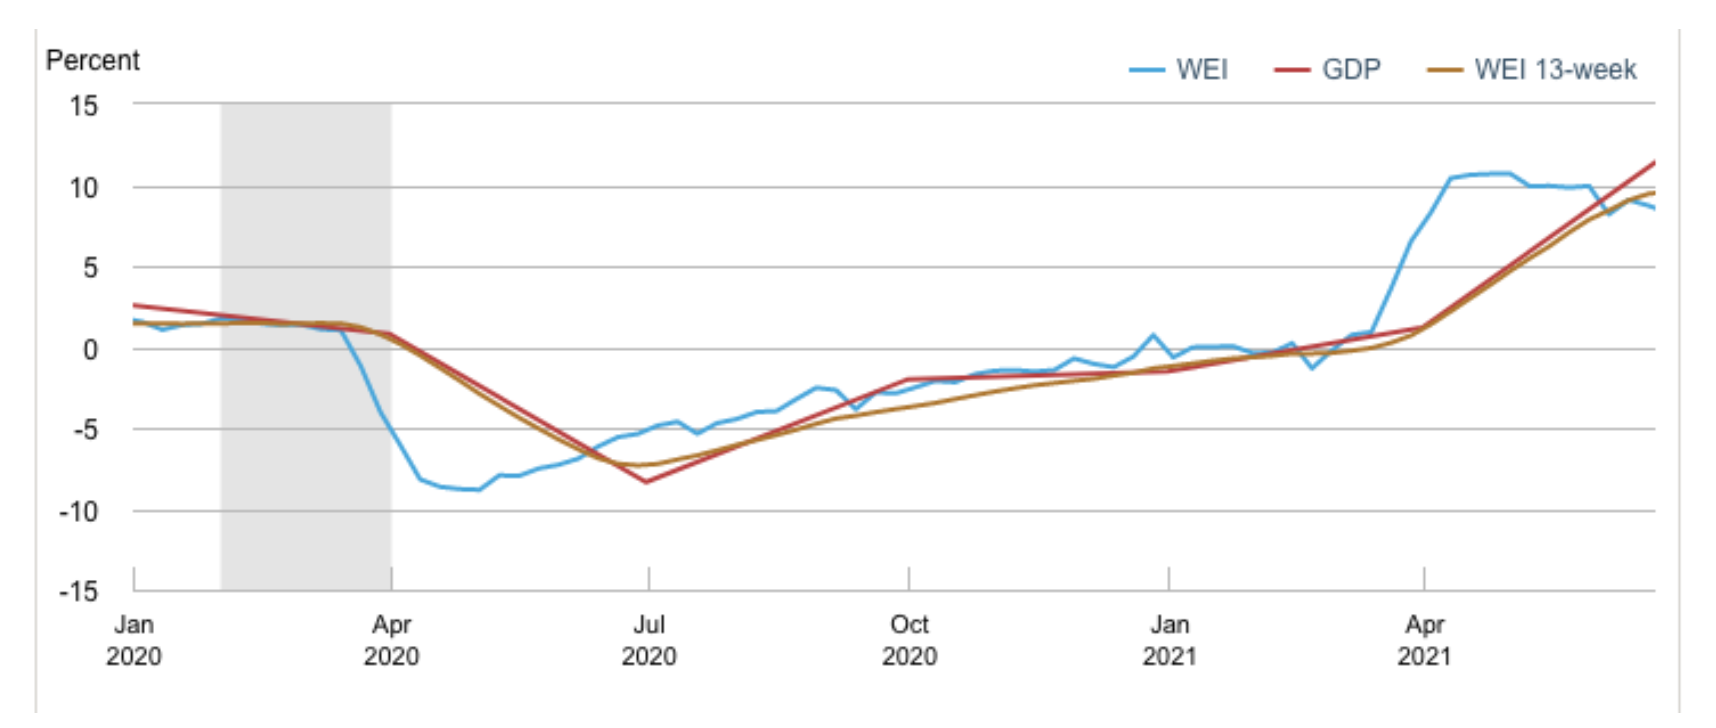
\includegraphics[width=4in]{images/ch7/weekly eco index.png}
            \caption{Weekly Economic Index (WEI) Nowcasts and Actual GDP}
        \end{figure}
        